%% ============================================================
%% sample.tex — チャプター追加・基本要素サンプル
%%
%% このファイルは stone-ship プロジェクトへの章追加方法を示す
%% サンプルドキュメントです．
%%
%% main.tex への組み込み方:
%%   %% ============================================================
%% sample.tex — チャプター追加・基本要素サンプル
%%
%% このファイルは stone-ship プロジェクトへの章追加方法を示す
%% サンプルドキュメントです．
%%
%% main.tex への組み込み方:
%%   %% ============================================================
%% sample.tex — チャプター追加・基本要素サンプル
%%
%% このファイルは stone-ship プロジェクトへの章追加方法を示す
%% サンプルドキュメントです．
%%
%% main.tex への組み込み方:
%%   %% ============================================================
%% sample.tex — チャプター追加・基本要素サンプル
%%
%% このファイルは stone-ship プロジェクトへの章追加方法を示す
%% サンプルドキュメントです．
%%
%% main.tex への組み込み方:
%%   \include{chapters/sample}  % 既に追加済み
%%   \include{chapters/yourchapter}
%%
%% 注意: 各章ファイルは \chapter{} から書き始め，
%%       文末に参考文献宣言を記述してください．
%% ============================================================

\chapter{章の追加方法（サンプル）}

この章は stone-ship プロジェクトに新しい章を追加する際の
基本的な使い方を示すサンプルです．

% ------------------------------------------------------------------
\section{ファイルの追加手順}
% ------------------------------------------------------------------

新しい章を追加するには，以下の手順に従ってください．

\begin{enumerate}
  \item \texttt{src/chapters/} 以下に \texttt{mychapter.tex} を作成する．
  \item ファイルの先頭を \verb|\chapter{章タイトル}| から書き始める．
  \item ファイル末尾に参考文献を宣言する（\ref{sec:bib} 節参照）．
  \item \texttt{src/main.tex} の \verb|\include| リストに追加する．
    \begin{itemize}
      \item 例: \verb|\include{chapters/mychapter}|
    \end{itemize}
  \item \texttt{utility/compile.sh} を実行してビルドする．
\end{enumerate}

% ------------------------------------------------------------------
\section{セクション構造}
% ------------------------------------------------------------------

章（\verb|\chapter|）の下には以下の見出しを使用できます．

\subsection{サブセクション}

\verb|\subsection{...}| で第2レベルの見出しを作ります．

\subsubsection{サブサブセクション}

\verb|\subsubsection{...}| で第3レベルの見出しを作ります．

必要に応じて \verb|\subsubsubsection|（paragraph）や
\verb|\subsubsubsubsection|（subparagraph）も利用できます
（\texttt{main.tex} で定義済み）．

% ------------------------------------------------------------------
\section{引用}
\label{sec:cite}
% ------------------------------------------------------------------

参考文献の引用には \texttt{natbib} パッケージの
\verb|\cite| と \verb|\citet| を使います．

\begin{itemize}
  \item \textbf{文末引用}: 文末で参照を示す場合 \verb|\cite{}| を使います\cite{Ben-Akiva1985}．
  \item \textbf{文中引用}: 著者名を文中に出す場合 \verb|\citet{}| を使います．
        例: \citet{Akamatsu1996} はマルコフ過程を用いた確率的交通量配分を提案した．
  \item \textbf{複数引用}: \verb|\cite{key1,key2}| で複数同時に引用できます
        \cite{Akamatsu1996,Ben-Akiva1985}．
\end{itemize}

% ------------------------------------------------------------------
\section{図}
\label{sec:fig}
% ------------------------------------------------------------------

図は \texttt{figure} 環境と \verb|\includegraphics| を使って挿入します（図\ref{fig:smpl-image}）．

\begin{figure}[hbtp]
  \centering
  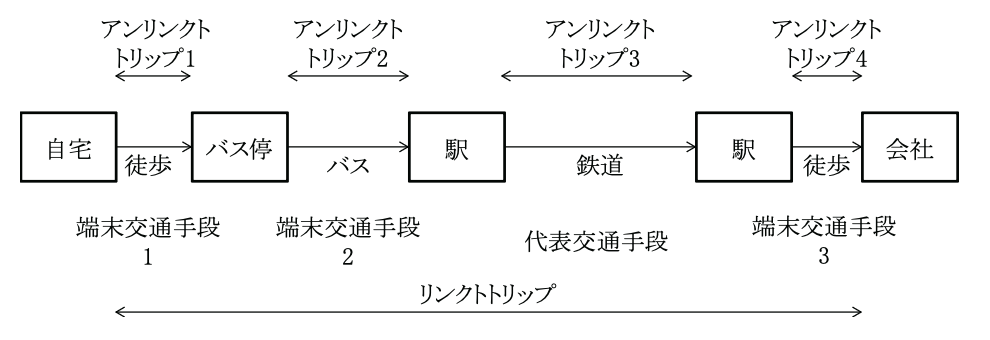
\includegraphics[width=0.6\textwidth]{assets/sample/sample.png}
  \caption{図のキャプション例．\texttt{assets/} フォルダに画像を置く．}
  \label{fig:smpl-image}
\end{figure}

\begin{itemize}
  \item 画像ファイルは \texttt{src/assets/} に配置します．
  \item \verb|[hbtp]| は配置オプション（here／bottom／top／page）です．
  \item \verb|\label{fig:xxx}| を設定すると \verb|\ref{fig:xxx}| で参照できます．
  \item PDF に変換するには PNG・PDF・EPS 形式を推奨します．
\end{itemize}

% ------------------------------------------------------------------
\section{表}
\label{sec:tab}
% ------------------------------------------------------------------

表は \texttt{table} 環境と \texttt{tabular} 環境を組み合わせます．
\texttt{booktabs} パッケージの罫線（表\ref{tab:smpl-data}）を推奨します．

\begin{table}[hbtp]
  \centering
  \caption{表のキャプション例（表番号の上に置く）．}
  \label{tab:smpl-data}
  \begin{tabular}{llr}
    \toprule
    変数名 & 説明 & 単位 \\
    \midrule
    $x$    & 距離 & km   \\
    $t$    & 時間 & 分   \\
    $c$    & 費用 & 円   \\
    \bottomrule
  \end{tabular}
\end{table}

\begin{itemize}
  \item \verb|\toprule| / \verb|\midrule| / \verb|\bottomrule| は
        \texttt{booktabs} の水平罫線です．
  \item キャプションは表の\textbf{上}，図の\textbf{下}に置くのが慣例です．
\end{itemize}

% ------------------------------------------------------------------
\section{数式}
\label{sec:math}
% ------------------------------------------------------------------

インライン数式は \verb|$...$|，ディスプレイ数式は \texttt{equation} 環境を使います．

二次方程式 $ax^2 + bx + c = 0$ の解は次式で与えられます：
\begin{equation}
  x = \frac{-b \pm \sqrt{b^2 - 4ac}}{2a}.
  \label{eq:quadratic}
\end{equation}

式\eqref{eq:quadratic}のように \verb|\label{}| と \verb|\eqref{}| で相互参照できます．

複数行の数式には \texttt{align} 環境を使います：
\begin{align}
  V_{ij} &= \beta_t t_{ij} + \beta_c c_{ij}, \label{eq:utility} \\
  P_{ij} &= \frac{\exp(V_{ij})}{\sum_k \exp(V_{ik})}. \label{eq:logit}
\end{align}

% ------------------------------------------------------------------
\section{ソースコード}
\label{sec:code}
% ------------------------------------------------------------------

ソースコードは \texttt{listings} + \texttt{jlisting} パッケージで挿入します
（リスト\ref{lst:sample}）．

\begin{lstlisting}[language=Python, caption={Pythonコードの例}, label={lst:sample}]
import numpy as np

def logit_prob(utilities):
    """ロジットモデルによる選択確率の計算."""
    exp_v = np.exp(utilities)
    return exp_v / exp_v.sum()

probs = logit_prob(np.array([-1.0, 0.5, 1.2]))
print(probs)
\end{lstlisting}

% ------------------------------------------------------------------
\section{相互参照まとめ}
% ------------------------------------------------------------------

\verb|\label{}| と \verb|\ref{}| / \verb|\eqref{}| を使って
ドキュメント内の任意の場所を参照できます（表\ref{tab:smpl-ref}）．

\begin{table}[hbtp]
  \centering
  \caption{相互参照の構文一覧．}
  \label{tab:smpl-ref}
  \begin{tabular}{lll}
    \toprule
    対象   & ラベル例               & 参照構文 \\
    \midrule
    章・節 & \texttt{sec:intro}     & \verb|\ref{sec:intro}| \\
    図     & \texttt{fig:result}    & \verb|\ref{fig:result}| \\
    表     & \texttt{tab:data}      & \verb|\ref{tab:data}| \\
    数式   & \texttt{eq:model}      & \verb|\eqref{eq:model}| \\
    コード & \texttt{lst:algorithm} & \verb|\ref{lst:algorithm}| \\
    \bottomrule
  \end{tabular}
\end{table}

% ------------------------------------------------------------------
\section{例題・コラム（tcolorbox）}
\label{sec:tcolorbox}
% ------------------------------------------------------------------

\texttt{tcolorbox} パッケージを使うと，色付きの枠で例題やコラムを表示できます．
プロジェクトでは \texttt{example} 環境（例題）と \texttt{column} 環境（コラム）が
\texttt{main.tex} で定義済みです．

\subsection{例題環境}

\verb|\begin{example}...\end{example}| で番号付きの例題ボックスを出力します
（\texttt{number within=chapter} により章番号と同期してリセットされます）．

\begin{example}
  二項ロジットモデルにおいて，代替案 $i$ の効用を $V_i$ とすると，
  選択確率は次式で表される：
  \begin{equation}
    P_i = \frac{\exp(V_i)}{\exp(V_1) + \exp(V_2)}.
  \end{equation}
  $V_1 = 1.0$，$V_2 = 0.5$ のとき，$P_1$ を求めよ．
\end{example}

\begin{example}[title={例題 \thetcbcounter（応用）}]
  \texttt{title=\{...\}} オプションを渡すとタイトルを上書きできます．
  \texttt{colback}（背景色）や \texttt{colframe}（枠色）も
  同様に個別指定が可能です．
\end{example}

\subsection{コラム環境}

\verb|\begin{column}{タイトル}...\end{column}| でタイトル付きのコラムを出力します．
例題と異なり番号は付きません．

\begin{column}{ロジットモデルの歴史}
  ロジットモデルは \citet{Ben-Akiva1985} らによって離散選択理論として体系化された．
  マルコフ過程への拡張については \citet{Akamatsu1996} を参照されたい．
\end{column}

\subsection{環境の定義（参考）}

\texttt{main.tex} 内の定義は以下のとおりです．
色や枠のスタイルを変更する場合はこれらを編集してください．

\begin{verbatim}
\usepackage[dvipdfmx]{tcolorbox}
\tcbuselibrary{breakable,skins}

\newtcolorbox[auto counter,number within=chapter]{example}[1][]{
  title={例題 \thetcbcounter},
  colback=blue!5!white, colframe=blue!40!black,
  fonttitle=\bfseries, breakable, #1
}

\newtcolorbox{column}[1]{
  title={コラム：#1},
  colback=gray!10!white, colframe=gray!50!black,
  fonttitle=\bfseries, breakable
}
\end{verbatim}

% ------------------------------------------------------------------
\section{参考文献の追加}
\label{sec:bib}
% ------------------------------------------------------------------

本プロジェクトでは \texttt{chapterbib} パッケージを使用しており，
参考文献リストは\textbf{章ごとに独立して}出力されます．
\textbf{bibファイルも章ごとに分けて管理}することを推奨します
（例: \texttt{1.bib}，\texttt{2.bib} など，章番号に対応したファイル名）．
こうすることで，各章の文献管理が独立し，共同編集時の競合を防げます．
新しい章を追加する際は，以下の手順で参考文献を設定してください．

\subsection{章ファイルへの参考文献宣言}

各章ファイルの\textbf{末尾}に必ず以下の3行を記述します．
\verb|\bibliography{}| には\textbf{その章専用の \texttt{.bib} ファイル}を指定します．

\begin{verbatim}
\addcontentsline{toc}{chapter}{参考文献}
\bibliographystyle{stone-ship}
\bibliography{../src/bibliography/mychapter}
\end{verbatim}

\begin{itemize}
  \item \verb|\addcontentsline{toc}{chapter}{参考文献}| は目次に「参考文献」を追加します．
  \item \verb|\bibliographystyle{stone-ship}| はプロジェクト独自のスタイルを指定します．
  \item \verb|\bibliography{../src/bibliography/mychapter}| は
        \textbf{この章専用の \texttt{.bib} ファイル}を指します
        （\texttt{src/} からの相対パスに \texttt{../src/} を付けた形式）．
  \item 複数ファイルを参照したい場合はカンマ区切りで指定できます．\\
        例: \verb|\bibliography{../src/bibliography/mychapter,|\\\hspace*{4.5em}\verb|../src/bibliography/shared}|
\end{itemize}

\subsection{bibファイルの作成・登録}

章ごとに \texttt{src/bibliography/} 以下に \texttt{.bib} ファイルを作成します．

\begin{enumerate}
  \item \texttt{src/bibliography/mychapter.bib} を新規作成する．
  \item 以下の形式でエントリを追記する（\texttt{@article}，\texttt{@book}，
        \texttt{@inproceedings} など）．
        \begin{verbatim}
@article{YourKey2025,
  author  = {Yamada, Taro},
  title   = {論文タイトル},
  journal = {ジャーナル名},
  volume  = {1},
  pages   = {1--10},
  year    = {2025}
}
        \end{verbatim}
  \item 日本語著者名はBibTeXが誤解析しないよう二重ブレースで囲む．\\
        例: \verb|author = {{山田太郎} and {鈴木次郎}}|
\end{enumerate}

\subsection{コンパイル}

\texttt{utility/compile.sh} を実行すると，
\texttt{build/chapters/} 以下に生成されたすべての章の \texttt{.aux} ファイルに対して
BibTeX が自動実行されるため，新しい章を追加しても \texttt{compile.sh} の編集は不要です．

% ==================================================================
% 参考文献（章の末尾に必ず記述）
% ==================================================================
\addcontentsline{toc}{chapter}{参考文献}
\bibliographystyle{stone-ship}
\bibliography{../src/bibliography/sample_refs}
  % 既に追加済み
%%   \include{chapters/yourchapter}
%%
%% 注意: 各章ファイルは \chapter{} から書き始め，
%%       文末に参考文献宣言を記述してください．
%% ============================================================

\chapter{章の追加方法（サンプル）}

この章は stone-ship プロジェクトに新しい章を追加する際の
基本的な使い方を示すサンプルです．

% ------------------------------------------------------------------
\section{ファイルの追加手順}
% ------------------------------------------------------------------

新しい章を追加するには，以下の手順に従ってください．

\begin{enumerate}
  \item \texttt{src/chapters/} 以下に \texttt{mychapter.tex} を作成する．
  \item ファイルの先頭を \verb|\chapter{章タイトル}| から書き始める．
  \item ファイル末尾に参考文献を宣言する（\ref{sec:bib} 節参照）．
  \item \texttt{src/main.tex} の \verb|\include| リストに追加する．
    \begin{itemize}
      \item 例: \verb|\include{chapters/mychapter}|
    \end{itemize}
  \item \texttt{utility/compile.sh} を実行してビルドする．
\end{enumerate}

% ------------------------------------------------------------------
\section{セクション構造}
% ------------------------------------------------------------------

章（\verb|\chapter|）の下には以下の見出しを使用できます．

\subsection{サブセクション}

\verb|\subsection{...}| で第2レベルの見出しを作ります．

\subsubsection{サブサブセクション}

\verb|\subsubsection{...}| で第3レベルの見出しを作ります．

必要に応じて \verb|\subsubsubsection|（paragraph）や
\verb|\subsubsubsubsection|（subparagraph）も利用できます
（\texttt{main.tex} で定義済み）．

% ------------------------------------------------------------------
\section{引用}
\label{sec:cite}
% ------------------------------------------------------------------

参考文献の引用には \texttt{natbib} パッケージの
\verb|\cite| と \verb|\citet| を使います．

\begin{itemize}
  \item \textbf{文末引用}: 文末で参照を示す場合 \verb|\cite{}| を使います\cite{Ben-Akiva1985}．
  \item \textbf{文中引用}: 著者名を文中に出す場合 \verb|\citet{}| を使います．
        例: \citet{Akamatsu1996} はマルコフ過程を用いた確率的交通量配分を提案した．
  \item \textbf{複数引用}: \verb|\cite{key1,key2}| で複数同時に引用できます
        \cite{Akamatsu1996,Ben-Akiva1985}．
\end{itemize}

% ------------------------------------------------------------------
\section{図}
\label{sec:fig}
% ------------------------------------------------------------------

図は \texttt{figure} 環境と \verb|\includegraphics| を使って挿入します（図\ref{fig:smpl-image}）．

\begin{figure}[hbtp]
  \centering
  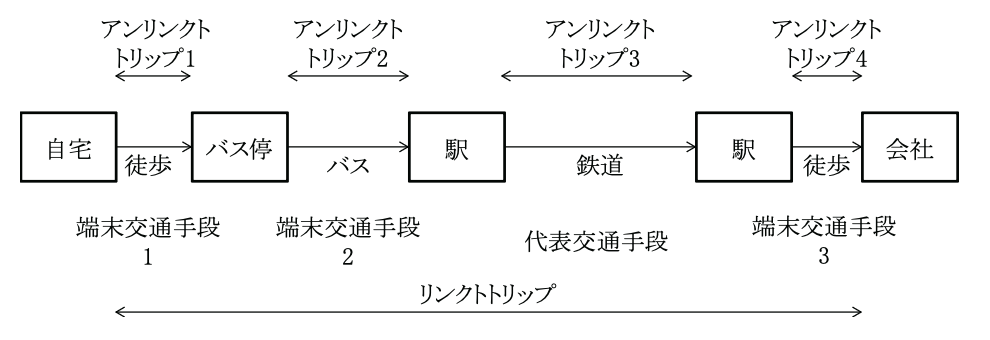
\includegraphics[width=0.6\textwidth]{assets/sample/sample.png}
  \caption{図のキャプション例．\texttt{assets/} フォルダに画像を置く．}
  \label{fig:smpl-image}
\end{figure}

\begin{itemize}
  \item 画像ファイルは \texttt{src/assets/} に配置します．
  \item \verb|[hbtp]| は配置オプション（here／bottom／top／page）です．
  \item \verb|\label{fig:xxx}| を設定すると \verb|\ref{fig:xxx}| で参照できます．
  \item PDF に変換するには PNG・PDF・EPS 形式を推奨します．
\end{itemize}

% ------------------------------------------------------------------
\section{表}
\label{sec:tab}
% ------------------------------------------------------------------

表は \texttt{table} 環境と \texttt{tabular} 環境を組み合わせます．
\texttt{booktabs} パッケージの罫線（表\ref{tab:smpl-data}）を推奨します．

\begin{table}[hbtp]
  \centering
  \caption{表のキャプション例（表番号の上に置く）．}
  \label{tab:smpl-data}
  \begin{tabular}{llr}
    \toprule
    変数名 & 説明 & 単位 \\
    \midrule
    $x$    & 距離 & km   \\
    $t$    & 時間 & 分   \\
    $c$    & 費用 & 円   \\
    \bottomrule
  \end{tabular}
\end{table}

\begin{itemize}
  \item \verb|\toprule| / \verb|\midrule| / \verb|\bottomrule| は
        \texttt{booktabs} の水平罫線です．
  \item キャプションは表の\textbf{上}，図の\textbf{下}に置くのが慣例です．
\end{itemize}

% ------------------------------------------------------------------
\section{数式}
\label{sec:math}
% ------------------------------------------------------------------

インライン数式は \verb|$...$|，ディスプレイ数式は \texttt{equation} 環境を使います．

二次方程式 $ax^2 + bx + c = 0$ の解は次式で与えられます：
\begin{equation}
  x = \frac{-b \pm \sqrt{b^2 - 4ac}}{2a}.
  \label{eq:quadratic}
\end{equation}

式\eqref{eq:quadratic}のように \verb|\label{}| と \verb|\eqref{}| で相互参照できます．

複数行の数式には \texttt{align} 環境を使います：
\begin{align}
  V_{ij} &= \beta_t t_{ij} + \beta_c c_{ij}, \label{eq:utility} \\
  P_{ij} &= \frac{\exp(V_{ij})}{\sum_k \exp(V_{ik})}. \label{eq:logit}
\end{align}

% ------------------------------------------------------------------
\section{ソースコード}
\label{sec:code}
% ------------------------------------------------------------------

ソースコードは \texttt{listings} + \texttt{jlisting} パッケージで挿入します
（リスト\ref{lst:sample}）．

\begin{lstlisting}[language=Python, caption={Pythonコードの例}, label={lst:sample}]
import numpy as np

def logit_prob(utilities):
    """ロジットモデルによる選択確率の計算."""
    exp_v = np.exp(utilities)
    return exp_v / exp_v.sum()

probs = logit_prob(np.array([-1.0, 0.5, 1.2]))
print(probs)
\end{lstlisting}

% ------------------------------------------------------------------
\section{相互参照まとめ}
% ------------------------------------------------------------------

\verb|\label{}| と \verb|\ref{}| / \verb|\eqref{}| を使って
ドキュメント内の任意の場所を参照できます（表\ref{tab:smpl-ref}）．

\begin{table}[hbtp]
  \centering
  \caption{相互参照の構文一覧．}
  \label{tab:smpl-ref}
  \begin{tabular}{lll}
    \toprule
    対象   & ラベル例               & 参照構文 \\
    \midrule
    章・節 & \texttt{sec:intro}     & \verb|\ref{sec:intro}| \\
    図     & \texttt{fig:result}    & \verb|\ref{fig:result}| \\
    表     & \texttt{tab:data}      & \verb|\ref{tab:data}| \\
    数式   & \texttt{eq:model}      & \verb|\eqref{eq:model}| \\
    コード & \texttt{lst:algorithm} & \verb|\ref{lst:algorithm}| \\
    \bottomrule
  \end{tabular}
\end{table}

% ------------------------------------------------------------------
\section{例題・コラム（tcolorbox）}
\label{sec:tcolorbox}
% ------------------------------------------------------------------

\texttt{tcolorbox} パッケージを使うと，色付きの枠で例題やコラムを表示できます．
プロジェクトでは \texttt{example} 環境（例題）と \texttt{column} 環境（コラム）が
\texttt{main.tex} で定義済みです．

\subsection{例題環境}

\verb|\begin{example}...\end{example}| で番号付きの例題ボックスを出力します
（\texttt{number within=chapter} により章番号と同期してリセットされます）．

\begin{example}
  二項ロジットモデルにおいて，代替案 $i$ の効用を $V_i$ とすると，
  選択確率は次式で表される：
  \begin{equation}
    P_i = \frac{\exp(V_i)}{\exp(V_1) + \exp(V_2)}.
  \end{equation}
  $V_1 = 1.0$，$V_2 = 0.5$ のとき，$P_1$ を求めよ．
\end{example}

\begin{example}[title={例題 \thetcbcounter（応用）}]
  \texttt{title=\{...\}} オプションを渡すとタイトルを上書きできます．
  \texttt{colback}（背景色）や \texttt{colframe}（枠色）も
  同様に個別指定が可能です．
\end{example}

\subsection{コラム環境}

\verb|\begin{column}{タイトル}...\end{column}| でタイトル付きのコラムを出力します．
例題と異なり番号は付きません．

\begin{column}{ロジットモデルの歴史}
  ロジットモデルは \citet{Ben-Akiva1985} らによって離散選択理論として体系化された．
  マルコフ過程への拡張については \citet{Akamatsu1996} を参照されたい．
\end{column}

\subsection{環境の定義（参考）}

\texttt{main.tex} 内の定義は以下のとおりです．
色や枠のスタイルを変更する場合はこれらを編集してください．

\begin{verbatim}
\usepackage[dvipdfmx]{tcolorbox}
\tcbuselibrary{breakable,skins}

\newtcolorbox[auto counter,number within=chapter]{example}[1][]{
  title={例題 \thetcbcounter},
  colback=blue!5!white, colframe=blue!40!black,
  fonttitle=\bfseries, breakable, #1
}

\newtcolorbox{column}[1]{
  title={コラム：#1},
  colback=gray!10!white, colframe=gray!50!black,
  fonttitle=\bfseries, breakable
}
\end{verbatim}

% ------------------------------------------------------------------
\section{参考文献の追加}
\label{sec:bib}
% ------------------------------------------------------------------

本プロジェクトでは \texttt{chapterbib} パッケージを使用しており，
参考文献リストは\textbf{章ごとに独立して}出力されます．
\textbf{bibファイルも章ごとに分けて管理}することを推奨します
（例: \texttt{1.bib}，\texttt{2.bib} など，章番号に対応したファイル名）．
こうすることで，各章の文献管理が独立し，共同編集時の競合を防げます．
新しい章を追加する際は，以下の手順で参考文献を設定してください．

\subsection{章ファイルへの参考文献宣言}

各章ファイルの\textbf{末尾}に必ず以下の3行を記述します．
\verb|\bibliography{}| には\textbf{その章専用の \texttt{.bib} ファイル}を指定します．

\begin{verbatim}
\addcontentsline{toc}{chapter}{参考文献}
\bibliographystyle{stone-ship}
\bibliography{../src/bibliography/mychapter}
\end{verbatim}

\begin{itemize}
  \item \verb|\addcontentsline{toc}{chapter}{参考文献}| は目次に「参考文献」を追加します．
  \item \verb|\bibliographystyle{stone-ship}| はプロジェクト独自のスタイルを指定します．
  \item \verb|\bibliography{../src/bibliography/mychapter}| は
        \textbf{この章専用の \texttt{.bib} ファイル}を指します
        （\texttt{src/} からの相対パスに \texttt{../src/} を付けた形式）．
  \item 複数ファイルを参照したい場合はカンマ区切りで指定できます．\\
        例: \verb|\bibliography{../src/bibliography/mychapter,|\\\hspace*{4.5em}\verb|../src/bibliography/shared}|
\end{itemize}

\subsection{bibファイルの作成・登録}

章ごとに \texttt{src/bibliography/} 以下に \texttt{.bib} ファイルを作成します．

\begin{enumerate}
  \item \texttt{src/bibliography/mychapter.bib} を新規作成する．
  \item 以下の形式でエントリを追記する（\texttt{@article}，\texttt{@book}，
        \texttt{@inproceedings} など）．
        \begin{verbatim}
@article{YourKey2025,
  author  = {Yamada, Taro},
  title   = {論文タイトル},
  journal = {ジャーナル名},
  volume  = {1},
  pages   = {1--10},
  year    = {2025}
}
        \end{verbatim}
  \item 日本語著者名はBibTeXが誤解析しないよう二重ブレースで囲む．\\
        例: \verb|author = {{山田太郎} and {鈴木次郎}}|
\end{enumerate}

\subsection{コンパイル}

\texttt{utility/compile.sh} を実行すると，
\texttt{build/chapters/} 以下に生成されたすべての章の \texttt{.aux} ファイルに対して
BibTeX が自動実行されるため，新しい章を追加しても \texttt{compile.sh} の編集は不要です．

% ==================================================================
% 参考文献（章の末尾に必ず記述）
% ==================================================================
\addcontentsline{toc}{chapter}{参考文献}
\bibliographystyle{stone-ship}
\bibliography{../src/bibliography/sample_refs}
  % 既に追加済み
%%   \include{chapters/yourchapter}
%%
%% 注意: 各章ファイルは \chapter{} から書き始め，
%%       文末に参考文献宣言を記述してください．
%% ============================================================

\chapter{章の追加方法（サンプル）}

この章は stone-ship プロジェクトに新しい章を追加する際の
基本的な使い方を示すサンプルです．

% ------------------------------------------------------------------
\section{ファイルの追加手順}
% ------------------------------------------------------------------

新しい章を追加するには，以下の手順に従ってください．

\begin{enumerate}
  \item \texttt{src/chapters/} 以下に \texttt{mychapter.tex} を作成する．
  \item ファイルの先頭を \verb|\chapter{章タイトル}| から書き始める．
  \item ファイル末尾に参考文献を宣言する（\ref{sec:bib} 節参照）．
  \item \texttt{src/main.tex} の \verb|\include| リストに追加する．
    \begin{itemize}
      \item 例: \verb|\include{chapters/mychapter}|
    \end{itemize}
  \item \texttt{utility/compile.sh} を実行してビルドする．
\end{enumerate}

% ------------------------------------------------------------------
\section{セクション構造}
% ------------------------------------------------------------------

章（\verb|\chapter|）の下には以下の見出しを使用できます．

\subsection{サブセクション}

\verb|\subsection{...}| で第2レベルの見出しを作ります．

\subsubsection{サブサブセクション}

\verb|\subsubsection{...}| で第3レベルの見出しを作ります．

必要に応じて \verb|\subsubsubsection|（paragraph）や
\verb|\subsubsubsubsection|（subparagraph）も利用できます
（\texttt{main.tex} で定義済み）．

% ------------------------------------------------------------------
\section{引用}
\label{sec:cite}
% ------------------------------------------------------------------

参考文献の引用には \texttt{natbib} パッケージの
\verb|\cite| と \verb|\citet| を使います．

\begin{itemize}
  \item \textbf{文末引用}: 文末で参照を示す場合 \verb|\cite{}| を使います\cite{Ben-Akiva1985}．
  \item \textbf{文中引用}: 著者名を文中に出す場合 \verb|\citet{}| を使います．
        例: \citet{Akamatsu1996} はマルコフ過程を用いた確率的交通量配分を提案した．
  \item \textbf{複数引用}: \verb|\cite{key1,key2}| で複数同時に引用できます
        \cite{Akamatsu1996,Ben-Akiva1985}．
\end{itemize}

% ------------------------------------------------------------------
\section{図}
\label{sec:fig}
% ------------------------------------------------------------------

図は \texttt{figure} 環境と \verb|\includegraphics| を使って挿入します（図\ref{fig:smpl-image}）．

\begin{figure}[hbtp]
  \centering
  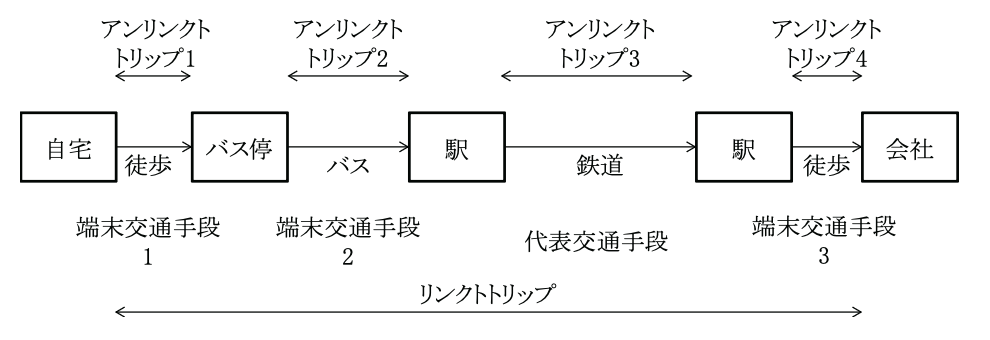
\includegraphics[width=0.6\textwidth]{assets/sample/sample.png}
  \caption{図のキャプション例．\texttt{assets/} フォルダに画像を置く．}
  \label{fig:smpl-image}
\end{figure}

\begin{itemize}
  \item 画像ファイルは \texttt{src/assets/} に配置します．
  \item \verb|[hbtp]| は配置オプション（here／bottom／top／page）です．
  \item \verb|\label{fig:xxx}| を設定すると \verb|\ref{fig:xxx}| で参照できます．
  \item PDF に変換するには PNG・PDF・EPS 形式を推奨します．
\end{itemize}

% ------------------------------------------------------------------
\section{表}
\label{sec:tab}
% ------------------------------------------------------------------

表は \texttt{table} 環境と \texttt{tabular} 環境を組み合わせます．
\texttt{booktabs} パッケージの罫線（表\ref{tab:smpl-data}）を推奨します．

\begin{table}[hbtp]
  \centering
  \caption{表のキャプション例（表番号の上に置く）．}
  \label{tab:smpl-data}
  \begin{tabular}{llr}
    \toprule
    変数名 & 説明 & 単位 \\
    \midrule
    $x$    & 距離 & km   \\
    $t$    & 時間 & 分   \\
    $c$    & 費用 & 円   \\
    \bottomrule
  \end{tabular}
\end{table}

\begin{itemize}
  \item \verb|\toprule| / \verb|\midrule| / \verb|\bottomrule| は
        \texttt{booktabs} の水平罫線です．
  \item キャプションは表の\textbf{上}，図の\textbf{下}に置くのが慣例です．
\end{itemize}

% ------------------------------------------------------------------
\section{数式}
\label{sec:math}
% ------------------------------------------------------------------

インライン数式は \verb|$...$|，ディスプレイ数式は \texttt{equation} 環境を使います．

二次方程式 $ax^2 + bx + c = 0$ の解は次式で与えられます：
\begin{equation}
  x = \frac{-b \pm \sqrt{b^2 - 4ac}}{2a}.
  \label{eq:quadratic}
\end{equation}

式\eqref{eq:quadratic}のように \verb|\label{}| と \verb|\eqref{}| で相互参照できます．

複数行の数式には \texttt{align} 環境を使います：
\begin{align}
  V_{ij} &= \beta_t t_{ij} + \beta_c c_{ij}, \label{eq:utility} \\
  P_{ij} &= \frac{\exp(V_{ij})}{\sum_k \exp(V_{ik})}. \label{eq:logit}
\end{align}

% ------------------------------------------------------------------
\section{ソースコード}
\label{sec:code}
% ------------------------------------------------------------------

ソースコードは \texttt{listings} + \texttt{jlisting} パッケージで挿入します
（リスト\ref{lst:sample}）．

\begin{lstlisting}[language=Python, caption={Pythonコードの例}, label={lst:sample}]
import numpy as np

def logit_prob(utilities):
    """ロジットモデルによる選択確率の計算."""
    exp_v = np.exp(utilities)
    return exp_v / exp_v.sum()

probs = logit_prob(np.array([-1.0, 0.5, 1.2]))
print(probs)
\end{lstlisting}

% ------------------------------------------------------------------
\section{相互参照まとめ}
% ------------------------------------------------------------------

\verb|\label{}| と \verb|\ref{}| / \verb|\eqref{}| を使って
ドキュメント内の任意の場所を参照できます（表\ref{tab:smpl-ref}）．

\begin{table}[hbtp]
  \centering
  \caption{相互参照の構文一覧．}
  \label{tab:smpl-ref}
  \begin{tabular}{lll}
    \toprule
    対象   & ラベル例               & 参照構文 \\
    \midrule
    章・節 & \texttt{sec:intro}     & \verb|\ref{sec:intro}| \\
    図     & \texttt{fig:result}    & \verb|\ref{fig:result}| \\
    表     & \texttt{tab:data}      & \verb|\ref{tab:data}| \\
    数式   & \texttt{eq:model}      & \verb|\eqref{eq:model}| \\
    コード & \texttt{lst:algorithm} & \verb|\ref{lst:algorithm}| \\
    \bottomrule
  \end{tabular}
\end{table}

% ------------------------------------------------------------------
\section{例題・コラム（tcolorbox）}
\label{sec:tcolorbox}
% ------------------------------------------------------------------

\texttt{tcolorbox} パッケージを使うと，色付きの枠で例題やコラムを表示できます．
プロジェクトでは \texttt{example} 環境（例題）と \texttt{column} 環境（コラム）が
\texttt{main.tex} で定義済みです．

\subsection{例題環境}

\verb|\begin{example}...\end{example}| で番号付きの例題ボックスを出力します
（\texttt{number within=chapter} により章番号と同期してリセットされます）．

\begin{example}
  二項ロジットモデルにおいて，代替案 $i$ の効用を $V_i$ とすると，
  選択確率は次式で表される：
  \begin{equation}
    P_i = \frac{\exp(V_i)}{\exp(V_1) + \exp(V_2)}.
  \end{equation}
  $V_1 = 1.0$，$V_2 = 0.5$ のとき，$P_1$ を求めよ．
\end{example}

\begin{example}[title={例題 \thetcbcounter（応用）}]
  \texttt{title=\{...\}} オプションを渡すとタイトルを上書きできます．
  \texttt{colback}（背景色）や \texttt{colframe}（枠色）も
  同様に個別指定が可能です．
\end{example}

\subsection{コラム環境}

\verb|\begin{column}{タイトル}...\end{column}| でタイトル付きのコラムを出力します．
例題と異なり番号は付きません．

\begin{column}{ロジットモデルの歴史}
  ロジットモデルは \citet{Ben-Akiva1985} らによって離散選択理論として体系化された．
  マルコフ過程への拡張については \citet{Akamatsu1996} を参照されたい．
\end{column}

\subsection{環境の定義（参考）}

\texttt{main.tex} 内の定義は以下のとおりです．
色や枠のスタイルを変更する場合はこれらを編集してください．

\begin{verbatim}
\usepackage[dvipdfmx]{tcolorbox}
\tcbuselibrary{breakable,skins}

\newtcolorbox[auto counter,number within=chapter]{example}[1][]{
  title={例題 \thetcbcounter},
  colback=blue!5!white, colframe=blue!40!black,
  fonttitle=\bfseries, breakable, #1
}

\newtcolorbox{column}[1]{
  title={コラム：#1},
  colback=gray!10!white, colframe=gray!50!black,
  fonttitle=\bfseries, breakable
}
\end{verbatim}

% ------------------------------------------------------------------
\section{参考文献の追加}
\label{sec:bib}
% ------------------------------------------------------------------

本プロジェクトでは \texttt{chapterbib} パッケージを使用しており，
参考文献リストは\textbf{章ごとに独立して}出力されます．
\textbf{bibファイルも章ごとに分けて管理}することを推奨します
（例: \texttt{1.bib}，\texttt{2.bib} など，章番号に対応したファイル名）．
こうすることで，各章の文献管理が独立し，共同編集時の競合を防げます．
新しい章を追加する際は，以下の手順で参考文献を設定してください．

\subsection{章ファイルへの参考文献宣言}

各章ファイルの\textbf{末尾}に必ず以下の3行を記述します．
\verb|\bibliography{}| には\textbf{その章専用の \texttt{.bib} ファイル}を指定します．

\begin{verbatim}
\addcontentsline{toc}{chapter}{参考文献}
\bibliographystyle{stone-ship}
\bibliography{../src/bibliography/mychapter}
\end{verbatim}

\begin{itemize}
  \item \verb|\addcontentsline{toc}{chapter}{参考文献}| は目次に「参考文献」を追加します．
  \item \verb|\bibliographystyle{stone-ship}| はプロジェクト独自のスタイルを指定します．
  \item \verb|\bibliography{../src/bibliography/mychapter}| は
        \textbf{この章専用の \texttt{.bib} ファイル}を指します
        （\texttt{src/} からの相対パスに \texttt{../src/} を付けた形式）．
  \item 複数ファイルを参照したい場合はカンマ区切りで指定できます．\\
        例: \verb|\bibliography{../src/bibliography/mychapter,|\\\hspace*{4.5em}\verb|../src/bibliography/shared}|
\end{itemize}

\subsection{bibファイルの作成・登録}

章ごとに \texttt{src/bibliography/} 以下に \texttt{.bib} ファイルを作成します．

\begin{enumerate}
  \item \texttt{src/bibliography/mychapter.bib} を新規作成する．
  \item 以下の形式でエントリを追記する（\texttt{@article}，\texttt{@book}，
        \texttt{@inproceedings} など）．
        \begin{verbatim}
@article{YourKey2025,
  author  = {Yamada, Taro},
  title   = {論文タイトル},
  journal = {ジャーナル名},
  volume  = {1},
  pages   = {1--10},
  year    = {2025}
}
        \end{verbatim}
  \item 日本語著者名はBibTeXが誤解析しないよう二重ブレースで囲む．\\
        例: \verb|author = {{山田太郎} and {鈴木次郎}}|
\end{enumerate}

\subsection{コンパイル}

\texttt{utility/compile.sh} を実行すると，
\texttt{build/chapters/} 以下に生成されたすべての章の \texttt{.aux} ファイルに対して
BibTeX が自動実行されるため，新しい章を追加しても \texttt{compile.sh} の編集は不要です．

% ==================================================================
% 参考文献（章の末尾に必ず記述）
% ==================================================================
\addcontentsline{toc}{chapter}{参考文献}
\bibliographystyle{stone-ship}
\bibliography{../src/bibliography/sample_refs}
  % 既に追加済み
%%   \include{chapters/yourchapter}
%%
%% 注意: 各章ファイルは \chapter{} から書き始め，
%%       文末に参考文献宣言を記述してください．
%% ============================================================

\chapter{章の追加方法（サンプル）}

この章は stone-ship プロジェクトに新しい章を追加する際の
基本的な使い方を示すサンプルです．

% ------------------------------------------------------------------
\section{ファイルの追加手順}
% ------------------------------------------------------------------

新しい章を追加するには，以下の手順に従ってください．

\begin{enumerate}
  \item \texttt{src/chapters/} 以下に \texttt{mychapter.tex} を作成する．
  \item ファイルの先頭を \verb|\chapter{章タイトル}| から書き始める．
  \item ファイル末尾に参考文献を宣言する（\ref{sec:bib} 節参照）．
  \item \texttt{src/main.tex} の \verb|\include| リストに追加する．
    \begin{itemize}
      \item 例: \verb|\include{chapters/mychapter}|
    \end{itemize}
  \item \texttt{utility/compile.sh} を実行してビルドする．
\end{enumerate}

% ------------------------------------------------------------------
\section{セクション構造}
% ------------------------------------------------------------------

章（\verb|\chapter|）の下には以下の見出しを使用できます．

\subsection{サブセクション}

\verb|\subsection{...}| で第2レベルの見出しを作ります．

\subsubsection{サブサブセクション}

\verb|\subsubsection{...}| で第3レベルの見出しを作ります．

必要に応じて \verb|\subsubsubsection|（paragraph）や
\verb|\subsubsubsubsection|（subparagraph）も利用できます
（\texttt{main.tex} で定義済み）．

% ------------------------------------------------------------------
\section{引用}
\label{sec:cite}
% ------------------------------------------------------------------

参考文献の引用には \texttt{natbib} パッケージの
\verb|\cite| と \verb|\citet| を使います．

\begin{itemize}
  \item \textbf{文末引用}: 文末で参照を示す場合 \verb|\cite{}| を使います\cite{Ben-Akiva1985}．
  \item \textbf{文中引用}: 著者名を文中に出す場合 \verb|\citet{}| を使います．
        例: \citet{Akamatsu1996} はマルコフ過程を用いた確率的交通量配分を提案した．
  \item \textbf{複数引用}: \verb|\cite{key1,key2}| で複数同時に引用できます
        \cite{Akamatsu1996,Ben-Akiva1985}．
\end{itemize}

% ------------------------------------------------------------------
\section{図}
\label{sec:fig}
% ------------------------------------------------------------------

図は \texttt{figure} 環境と \verb|\includegraphics| を使って挿入します（図\ref{fig:smpl-image}）．

\begin{figure}[hbtp]
  \centering
  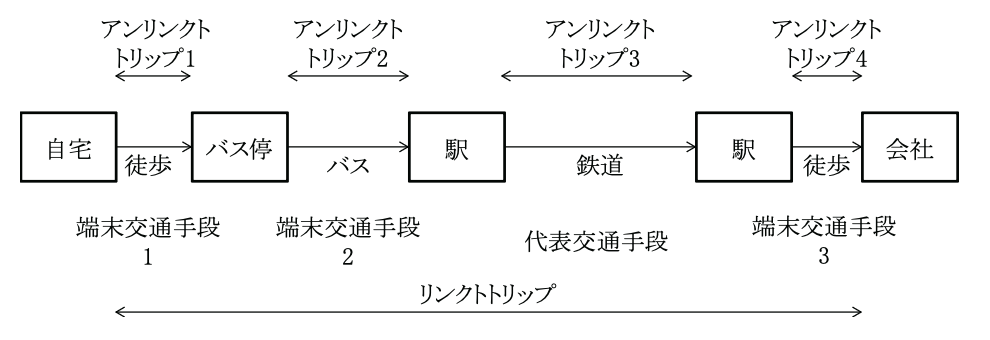
\includegraphics[width=0.6\textwidth]{assets/sample/sample.png}
  \caption{図のキャプション例．\texttt{assets/} フォルダに画像を置く．}
  \label{fig:smpl-image}
\end{figure}

\begin{itemize}
  \item 画像ファイルは \texttt{src/assets/} に配置します．
  \item \verb|[hbtp]| は配置オプション（here／bottom／top／page）です．
  \item \verb|\label{fig:xxx}| を設定すると \verb|\ref{fig:xxx}| で参照できます．
  \item PDF に変換するには PNG・PDF・EPS 形式を推奨します．
\end{itemize}

% ------------------------------------------------------------------
\section{表}
\label{sec:tab}
% ------------------------------------------------------------------

表は \texttt{table} 環境と \texttt{tabular} 環境を組み合わせます．
\texttt{booktabs} パッケージの罫線（表\ref{tab:smpl-data}）を推奨します．

\begin{table}[hbtp]
  \centering
  \caption{表のキャプション例（表番号の上に置く）．}
  \label{tab:smpl-data}
  \begin{tabular}{llr}
    \toprule
    変数名 & 説明 & 単位 \\
    \midrule
    $x$    & 距離 & km   \\
    $t$    & 時間 & 分   \\
    $c$    & 費用 & 円   \\
    \bottomrule
  \end{tabular}
\end{table}

\begin{itemize}
  \item \verb|\toprule| / \verb|\midrule| / \verb|\bottomrule| は
        \texttt{booktabs} の水平罫線です．
  \item キャプションは表の\textbf{上}，図の\textbf{下}に置くのが慣例です．
\end{itemize}

% ------------------------------------------------------------------
\section{数式}
\label{sec:math}
% ------------------------------------------------------------------

インライン数式は \verb|$...$|，ディスプレイ数式は \texttt{equation} 環境を使います．

二次方程式 $ax^2 + bx + c = 0$ の解は次式で与えられます：
\begin{equation}
  x = \frac{-b \pm \sqrt{b^2 - 4ac}}{2a}.
  \label{eq:quadratic}
\end{equation}

式\eqref{eq:quadratic}のように \verb|\label{}| と \verb|\eqref{}| で相互参照できます．

複数行の数式には \texttt{align} 環境を使います：
\begin{align}
  V_{ij} &= \beta_t t_{ij} + \beta_c c_{ij}, \label{eq:utility} \\
  P_{ij} &= \frac{\exp(V_{ij})}{\sum_k \exp(V_{ik})}. \label{eq:logit}
\end{align}

% ------------------------------------------------------------------
\section{ソースコード}
\label{sec:code}
% ------------------------------------------------------------------

ソースコードは \texttt{listings} + \texttt{jlisting} パッケージで挿入します
（リスト\ref{lst:sample}）．

\begin{lstlisting}[language=Python, caption={Pythonコードの例}, label={lst:sample}]
import numpy as np

def logit_prob(utilities):
    """ロジットモデルによる選択確率の計算."""
    exp_v = np.exp(utilities)
    return exp_v / exp_v.sum()

probs = logit_prob(np.array([-1.0, 0.5, 1.2]))
print(probs)
\end{lstlisting}

% ------------------------------------------------------------------
\section{相互参照まとめ}
% ------------------------------------------------------------------

\verb|\label{}| と \verb|\ref{}| / \verb|\eqref{}| を使って
ドキュメント内の任意の場所を参照できます（表\ref{tab:smpl-ref}）．

\begin{table}[hbtp]
  \centering
  \caption{相互参照の構文一覧．}
  \label{tab:smpl-ref}
  \begin{tabular}{lll}
    \toprule
    対象   & ラベル例               & 参照構文 \\
    \midrule
    章・節 & \texttt{sec:intro}     & \verb|\ref{sec:intro}| \\
    図     & \texttt{fig:result}    & \verb|\ref{fig:result}| \\
    表     & \texttt{tab:data}      & \verb|\ref{tab:data}| \\
    数式   & \texttt{eq:model}      & \verb|\eqref{eq:model}| \\
    コード & \texttt{lst:algorithm} & \verb|\ref{lst:algorithm}| \\
    \bottomrule
  \end{tabular}
\end{table}

% ------------------------------------------------------------------
\section{例題・コラム（tcolorbox）}
\label{sec:tcolorbox}
% ------------------------------------------------------------------

\texttt{tcolorbox} パッケージを使うと，色付きの枠で例題やコラムを表示できます．
プロジェクトでは \texttt{example} 環境（例題）と \texttt{column} 環境（コラム）が
\texttt{main.tex} で定義済みです．

\subsection{例題環境}

\verb|\begin{example}...\end{example}| で番号付きの例題ボックスを出力します
（\texttt{number within=chapter} により章番号と同期してリセットされます）．

\begin{example}
  二項ロジットモデルにおいて，代替案 $i$ の効用を $V_i$ とすると，
  選択確率は次式で表される：
  \begin{equation}
    P_i = \frac{\exp(V_i)}{\exp(V_1) + \exp(V_2)}.
  \end{equation}
  $V_1 = 1.0$，$V_2 = 0.5$ のとき，$P_1$ を求めよ．
\end{example}

\begin{example}[title={例題 \thetcbcounter（応用）}]
  \texttt{title=\{...\}} オプションを渡すとタイトルを上書きできます．
  \texttt{colback}（背景色）や \texttt{colframe}（枠色）も
  同様に個別指定が可能です．
\end{example}

\subsection{コラム環境}

\verb|\begin{column}{タイトル}...\end{column}| でタイトル付きのコラムを出力します．
例題と異なり番号は付きません．

\begin{column}{ロジットモデルの歴史}
  ロジットモデルは \citet{Ben-Akiva1985} らによって離散選択理論として体系化された．
  マルコフ過程への拡張については \citet{Akamatsu1996} を参照されたい．
\end{column}

\subsection{環境の定義（参考）}

\texttt{main.tex} 内の定義は以下のとおりです．
色や枠のスタイルを変更する場合はこれらを編集してください．

\begin{verbatim}
\usepackage[dvipdfmx]{tcolorbox}
\tcbuselibrary{breakable,skins}

\newtcolorbox[auto counter,number within=chapter]{example}[1][]{
  title={例題 \thetcbcounter},
  colback=blue!5!white, colframe=blue!40!black,
  fonttitle=\bfseries, breakable, #1
}

\newtcolorbox{column}[1]{
  title={コラム：#1},
  colback=gray!10!white, colframe=gray!50!black,
  fonttitle=\bfseries, breakable
}
\end{verbatim}

% ------------------------------------------------------------------
\section{参考文献の追加}
\label{sec:bib}
% ------------------------------------------------------------------

本プロジェクトでは \texttt{chapterbib} パッケージを使用しており，
参考文献リストは\textbf{章ごとに独立して}出力されます．
\textbf{bibファイルも章ごとに分けて管理}することを推奨します
（例: \texttt{1.bib}，\texttt{2.bib} など，章番号に対応したファイル名）．
こうすることで，各章の文献管理が独立し，共同編集時の競合を防げます．
新しい章を追加する際は，以下の手順で参考文献を設定してください．

\subsection{章ファイルへの参考文献宣言}

各章ファイルの\textbf{末尾}に必ず以下の3行を記述します．
\verb|\bibliography{}| には\textbf{その章専用の \texttt{.bib} ファイル}を指定します．

\begin{verbatim}
\addcontentsline{toc}{chapter}{参考文献}
\bibliographystyle{stone-ship}
\bibliography{../src/bibliography/mychapter}
\end{verbatim}

\begin{itemize}
  \item \verb|\addcontentsline{toc}{chapter}{参考文献}| は目次に「参考文献」を追加します．
  \item \verb|\bibliographystyle{stone-ship}| はプロジェクト独自のスタイルを指定します．
  \item \verb|\bibliography{../src/bibliography/mychapter}| は
        \textbf{この章専用の \texttt{.bib} ファイル}を指します
        （\texttt{src/} からの相対パスに \texttt{../src/} を付けた形式）．
  \item 複数ファイルを参照したい場合はカンマ区切りで指定できます．\\
        例: \verb|\bibliography{../src/bibliography/mychapter,|\\\hspace*{4.5em}\verb|../src/bibliography/shared}|
\end{itemize}

\subsection{bibファイルの作成・登録}

章ごとに \texttt{src/bibliography/} 以下に \texttt{.bib} ファイルを作成します．

\begin{enumerate}
  \item \texttt{src/bibliography/mychapter.bib} を新規作成する．
  \item 以下の形式でエントリを追記する（\texttt{@article}，\texttt{@book}，
        \texttt{@inproceedings} など）．
        \begin{verbatim}
@article{YourKey2025,
  author  = {Yamada, Taro},
  title   = {論文タイトル},
  journal = {ジャーナル名},
  volume  = {1},
  pages   = {1--10},
  year    = {2025}
}
        \end{verbatim}
  \item 日本語著者名はBibTeXが誤解析しないよう二重ブレースで囲む．\\
        例: \verb|author = {{山田太郎} and {鈴木次郎}}|
\end{enumerate}

\subsection{コンパイル}

\texttt{utility/compile.sh} を実行すると，
\texttt{build/chapters/} 以下に生成されたすべての章の \texttt{.aux} ファイルに対して
BibTeX が自動実行されるため，新しい章を追加しても \texttt{compile.sh} の編集は不要です．

% ==================================================================
% 参考文献（章の末尾に必ず記述）
% ==================================================================
\addcontentsline{toc}{chapter}{参考文献}
\bibliographystyle{stone-ship}
\bibliography{../src/bibliography/sample_refs}
